\documentclass[letterpaper]{article}
\usepackage[submission]{aaai2027}
\usepackage[hyphens]{url}
\usepackage{graphicx}
\urlstyle{rm}
\def\UrlFont{\rm}
\usepackage{natbib}
\usepackage{caption}
\usepackage{booktabs}
\frenchspacing
\pdfinfo{
/TemplateVersion (2027.1)
}

\setcounter{secnumdepth}{0}

\title{Optim-Agent: LLM Agents as Your Hyperparameter Optimizer}
\author{Anonymous Submission}
\affiliations{}

\begin{document}
\maketitle

\begin{abstract}
Hyperparameter optimization (HPO) is usually treated as a black-box numerical
problem, even though practitioners routinely exploit semantic knowledge about
what each knob controls. We present \emph{optim-agent}, a Python package that
turns an existing command-line LLM agent into a drop-in sampler and pruner for
machine-learning training loops. Instead of fitting a surrogate alone, the
agent receives the search space, typed parameter context, and trial history,
then proposes the next configuration through a standard ask--tell study API.
This design lets the optimizer combine quantitative trends with qualitative
priors such as ``large learning rates destabilize small batches'' while keeping
runtime dependencies minimal. Across analytic functions, MNIST, CIFAR-10, and
ablation studies, agent-guided sampling is strongest in the small-budget regime
where classical methods have little data: GPT-5.5 and Opus-4.8 solve Branin and
Ackley within ten trials; higher Codex reasoning effort improves CIFAR-10 from
28.50\% to 26.50\% test error; and moderate agent pruning saves synthetic
compute without sacrificing the optimum. The package requires no hosted service
beyond the user's authenticated CLI, stores studies in JSON or SQLite, and keeps
all experiments reproducible in the public examples directory.
\end{abstract}

\section{Introduction}

HPO is a central bottleneck in empirical AI. Random search is simple and often
competitive when only a few dimensions matter \cite{bergstra2012random}, while
Bayesian optimization and TPE become powerful once enough observations support a
useful surrogate \cite{snoek2012practical,akiba2019optuna}. Yet the first
several trials of a real training run are not purely numerical. A practitioner
knows that learning rate, batch size, dropout, weight decay, augmentation
strength, model width, and optimizer schedule have meanings; a failed high
learning rate suggests a different response than a failed crop-padding value.
Classical black-box optimizers generally ignore this language-level structure.

Large language model agents introduce a different computational object: a model
that can read a natural-language description, inspect a short history, and act
through a tool interface \cite{brown2020language,yao2023react,wang2024surveyagents}.
The question is whether that capability can be made useful for HPO without
turning every training run into a bespoke prompt-engineering project. We answer
yes through \emph{optim-agent}, an installable Python package whose sampler
delegates the ``choose the next point'' step to an existing CLI agent such as
Codex, Claude Code, or OpenCode. The user writes the same define-by-run
objective used by Optuna-style frameworks, but may attach semantic context to
each parameter.

Our contribution is practical and empirical. First, we define a dependency-light
study API in which LLM agents act as samplers and optional pruners. Second, we
show how sampler effort controls history length, explicit reasoning, persistent
notes, and ranked candidates. Third, we evaluate the package on analytic and
vision benchmarks using the experiment scripts in \texttt{examples/} and the
logged artifacts in \texttt{docs/assets/}. The results indicate that agent HPO
is not a universal replacement for mature Bayesian or bandit methods, but it is
especially attractive when trial budgets are small, objectives are expensive,
and hyperparameters have domain semantics.

\section{Related Work}

Classical HPO spans random search, Bayesian optimization, multi-fidelity
bandits, evolutionary search, and automated machine learning systems
\cite{bergstra2012random,snoek2012practical,li2017hyperband,falkner2018bohb,feurer2015autosklearn,hutter2019automl}.
These methods deliberately treat the objective as a black box and derive sample
efficiency from statistical structure. Neural architecture search extends the
same automation impulse to model topology \cite{elsken2019nas}. \emph{optim-agent}
does not compete with these methods by proposing a new surrogate. Instead, it
adds a language-conditioned sampler that can be used through the same objective
interface and compared against TPE and random search.

LLM-agent research studies systems that reason, call tools, keep memory, and
act in external environments \cite{yao2023react,wang2024surveyagents}. Those
ideas are usually evaluated on software tasks, web interaction, or planning.
Here the environment is an HPO study: the agent sees a compact table of trials
and returns JSON parameters. This narrower interface is useful because every
agent action has a mechanical consequence: the training objective either
improves or it does not.

\section{Method}

\textbf{Study API.} The package exposes \texttt{create\_study},
\texttt{Trial.suggest\_*}, \texttt{Study.optimize}, and an ask--tell path for
session-driven use. Search distributions include floats, integers, and
categoricals, each optionally annotated with natural-language context. A study
can persist to JSON for single-writer runs or SQLite for concurrent workers.

\textbf{AgentSampler.} At each non-warmup trial, the sampler serializes the
search space, parameter meanings, objective direction, and recent trial history.
The agent is instructed to return only a JSON object containing candidate values.
The package validates each value against the registered distribution, clamps
numeric outliers, rejects invalid categoricals, and falls back to random sampling
if the agent call fails. This makes the LLM advisory rather than trusted.

\begin{table}[t]
\centering
\begin{tabular}{lcccc}
\toprule
Effort & History & Reason & Notes & Candidates \\
\midrule
low & 5 & no & no & 1 \\
medium & 15 & no & no & 1 \\
high & all & yes & no & 1 \\
xhigh & all & yes & yes & 1 \\
max & all & yes & yes & 3 \\
\bottomrule
\end{tabular}
\caption{AgentSampler effort levels. ``All'' history is capped in the implementation
to avoid oversized prompts.}
\label{tab:effort}
\end{table}

\textbf{AgentPruner.} The optional pruner compares an in-progress learning
curve with the best completed trials. Levels \emph{loose}, \emph{medium}, and
\emph{tight} vary warmup fraction and consultation interval. On agent failure,
the pruner keeps the trial to avoid losing data through infrastructure noise.

\textbf{Skill mode.} The package black-box API is complemented by an agent skill:
a coding agent can read the target project, choose explicit parameters through
\texttt{study.ask(params)}, run the user's training command, and record the
result with \texttt{study.tell}. This path is useful when the source code itself
explains hidden constraints that are too cumbersome to encode in a search-space
description.

\section{Experiments}

All experiment code remains in \texttt{examples/}. We use
\texttt{examples/hard\_functions.py} for analytic functions,
\texttt{examples/mnist.py} for MNIST, \texttt{examples/cifar10.py} for CIFAR-10,
and \texttt{examples/ablations.py} for effort and pruning ablations. The plotted
curves and JSON trial logs are stored in \texttt{docs/assets/}. Unless stated
otherwise, lower is better and curves report best value so far.

\subsection{Analytic Functions}

The Branin 2D and Ackley 5D tests isolate sample efficiency. Agents are told
only input bounds and trial history, never the function name, optimum location,
or optimum value. Each method receives ten trials over three seeds.

\begin{figure*}[t]
\centering
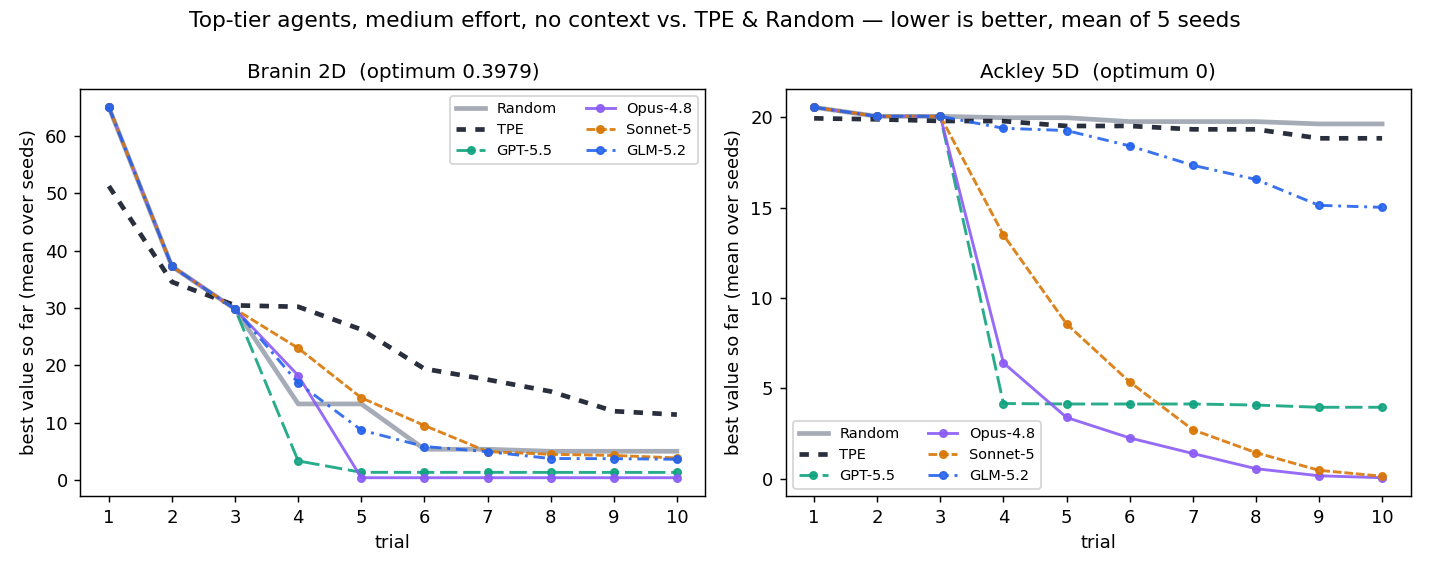
\includegraphics[width=.48\textwidth]{../../docs/assets/hard_benchmarks_tier.png}
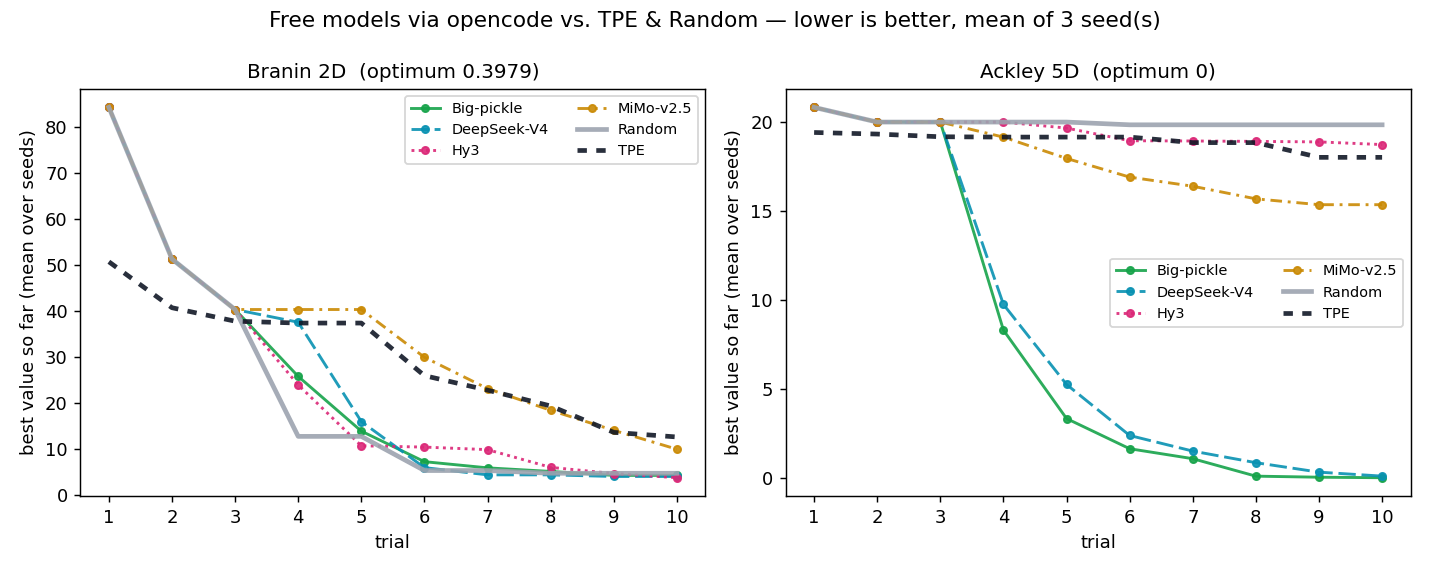
\includegraphics[width=.48\textwidth]{../../docs/assets/hard_benchmarks_free.png}
\caption{Analytic-function benchmarks from \texttt{examples/hard\_functions.py}.
Left: headline agents. Right: free OpenCode models.}
\label{fig:hard}
\end{figure*}

\begin{table}[t]
\centering
\begin{tabular}{lcc}
\toprule
Method & Branin & Ackley-5D \\
\midrule
Opus-4.8 & \textbf{0.40} & \textbf{0.00} \\
GPT-5.5 & \textbf{0.40} & \textbf{0.00} \\
GLM-5.2 & 4.26 & \textbf{0.00} \\
Big-pickle & 4.26 & \textbf{0.00} \\
DeepSeek-V4 & 4.02 & 0.09 \\
Random & 4.72 & 19.83 \\
TPE & 12.60 & 18.00 \\
\bottomrule
\end{tabular}
\caption{Best value after ten trials, mean over three seeds. Branin optimum is
approximately 0.398; Ackley optimum is 0.}
\label{tab:hard}
\end{table}

Table~\ref{tab:hard} shows the low-budget pattern. The strongest agents reach
both optima, while TPE has too little data to build a useful density model.
Several free OpenCode models also solve Ackley, suggesting that the interface
does not require a proprietary frontier model for every objective.

\subsection{MNIST and CIFAR-10}

MNIST uses a small CNN/ResNet-style classifier on full train/test splits, with
24 trials, three seeds, and three epochs per trial. The search space includes
learning rate, batch size, dropout, width, depth, shift, and rotation. CIFAR-10
uses a small ResNet with 12 trials, three seeds, and a wider space including
weight decay, depth, label smoothing, crop padding, and horizontal flip
probability \cite{leCun1998mnist,krizhevsky2009cifar}. Trials were parallelized
across eight GPUs as recorded by the JSON logs.

\begin{figure*}[t]
\centering
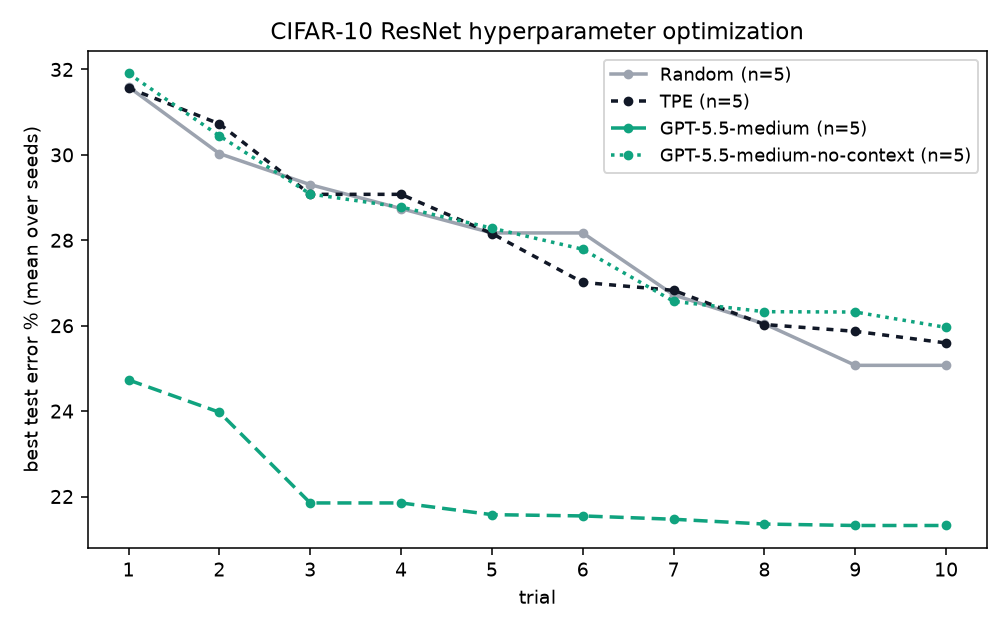
\includegraphics[width=.48\textwidth]{../../docs/assets/cifar10_benchmarks.png}
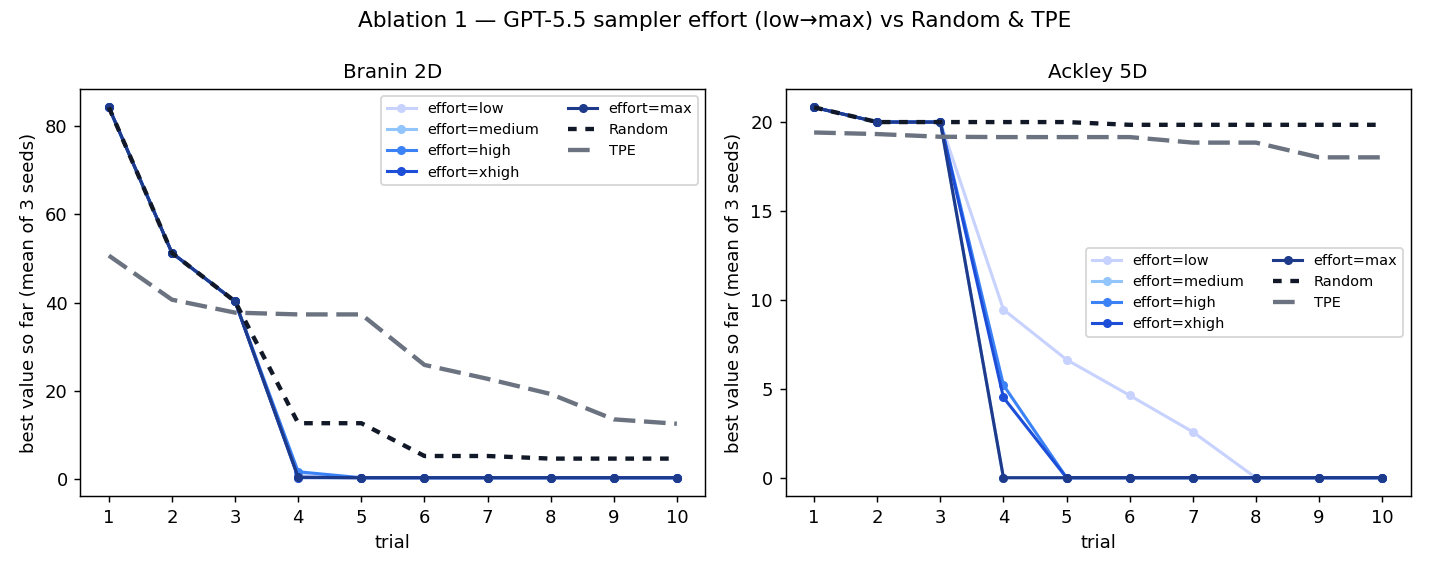
\includegraphics[width=.48\textwidth]{../../docs/assets/abl_effort.png}
\caption{Left: CIFAR-10 effort sweep from \texttt{examples/cifar10.py}. Right:
analytic effort ablation from \texttt{examples/ablations.py}.}
\label{fig:cifar-effort}
\end{figure*}

\begin{table}[t]
\centering
\begin{tabular}{lcc}
\toprule
Method & MNIST err. & CIFAR-10 err. \\
\midrule
Random & 0.51\% & 28.06\% \\
TPE & 0.56\% & 28.14\% \\
GPT-5.5 low & 0.53\% & 28.50\% \\
GPT-5.5 medium & 0.51\% & 27.10\% \\
GPT-5.5 xhigh & 0.52\% & \textbf{26.50\%} \\
\bottomrule
\end{tabular}
\caption{Mean best test error over three seeds from the current JSON logs.
CIFAR-10 rewards higher effort most clearly.}
\label{tab:vision}
\end{table}

The MNIST task is nearly saturated: random search is already strong, and agent
effort separates only weakly. CIFAR-10 is more informative. The xhigh sampler
improves mean best error to 26.50\%, ahead of medium at 27.10\%, random at
28.06\%, and TPE at 28.14\%. This is the regime where the agent's qualitative
priors over optimization and augmentation appear useful.

\subsection{Ablations}

\begin{figure}[t]
\centering
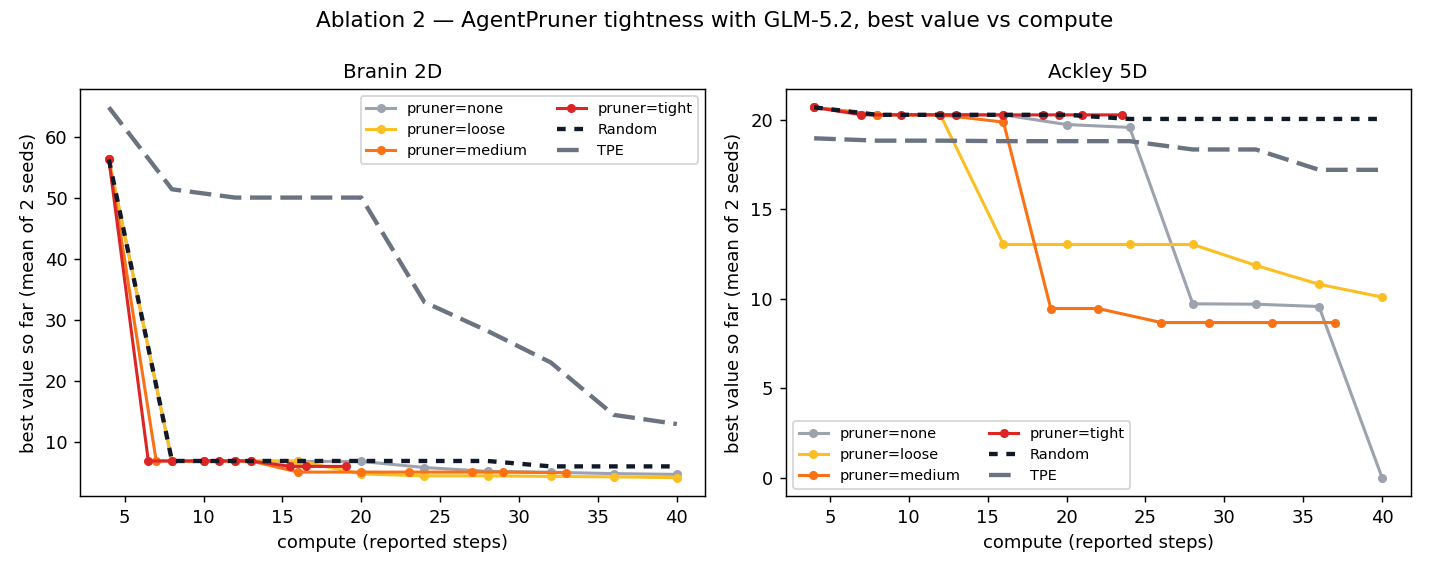
\includegraphics[width=\columnwidth]{../../docs/assets/abl_prune.png}
\caption{AgentPruner tightness ablation. Moderate pruning saves reported steps;
tight pruning stops too aggressively.}
\label{fig:prune}
\end{figure}

The effort ablation fixes the model to GPT-5.5/Codex and varies the sampler
settings in Table~\ref{tab:effort}. On Branin/Ackley, every effort reaches the
optimum, indicating that the benchmark is too easy to separate reasoning depth.
However, the CIFAR-10 sweep shows a monotone gain from low to xhigh.

The pruning ablation adds synthetic four-step learning curves to analytic
function values so that a pruner has intermediate evidence. Loose and medium
pruning reach near-optimal final values with fewer reported steps than no
pruning; tight pruning averages roughly 17.5 steps but stalls around Branin
6.86 and Ackley 20.35. The practical recommendation is therefore conservative:
use pruning when trial cost is high, and prefer loose or medium settings unless
early stopping false positives are acceptable.

\section{Discussion}

Agent HPO is most compelling when three conditions hold. First, each objective
evaluation is expensive enough that one agent call is cheap by comparison.
Second, the search budget is small enough that classical surrogates are still
data-starved. Third, the knobs have semantics that can be described in language.
The analytic results isolate the small-budget effect; the CIFAR-10 sweep shows
the semantic and reasoning-effort effect on a real training task.

The package deliberately avoids hiding failures. Invalid JSON, out-of-range
values, backend timeouts, and pruner errors fall back to conservative behavior.
This choice lowers peak cleverness but makes the system usable in ordinary
training loops. The SQLite backend also makes parallel studies boring: workers
communicate through the database rather than a custom scheduler.

\section{Limitations and Broader Impact}

The empirical study is still modest. Three seeds quantify variation only
coarsely, and no claim of universal dominance is warranted. Some results depend
on particular CLI model versions, and free model rosters may change. Agent
sampling can also consume paid tokens and may leak sensitive parameter names or
trial summaries if used with remote backends; users should avoid sending private
data to untrusted services. The positive impact is broader access to practical
HPO: students and small labs can run free or local agent backends, and the
package keeps random and TPE baselines available for comparison.

\section{Reproducibility}

The package itself has zero runtime dependencies beyond Python's standard
library; the experiment extra installs NumPy, Matplotlib, and Optuna for
plotting and TPE. Tests run with \texttt{python3 tests/test\_optim\_agent.py}.
Analytic figures can be regenerated by running
\texttt{python examples/hard\_functions.py plot}; ablations by
\texttt{python examples/ablations.py plot}; and full benchmark runs by the
\texttt{run} subcommands in each example script. The JSON logs in
\texttt{docs/assets/} record seeds, best values, parameters, GPU lists, trial
counts, and worker counts. MNIST was run on eight A800 GPUs in the recorded
README, while CIFAR-10 was run on eight A100 GPUs; both use full public datasets
and fixed seed lists 0, 1, and 2. No new dataset is introduced.

\section{Conclusion}

\emph{optim-agent} makes LLM agents a small, inspectable component in the HPO
loop: read the search space, reason over trial history, propose JSON, validate,
and fall back safely. The results support a bounded claim: agent samplers can be
highly sample-efficient in small-budget settings and can improve real training
tasks when parameter semantics matter. The package gives researchers a simple
way to test that claim in their own objectives without abandoning familiar HPO
interfaces.

\bibliography{optim-agent}

\end{document}
